\documentclass[xcolor=svgnames]{beamer}
\usecolortheme[named=Teal]{structure}
\useoutertheme{infolines}
\usetheme{Rochester}
\setbeamertemplate{navigation symbols}{}


\usepackage{graphicx}
\usepackage{array}
\usepackage{subfigure}
\usepackage{verbatim}


%commands
\def\CPP{{C\kern-.05em\raise.23ex\hbox{+\kern-.05em+}}}
\newcommand{\tr}[1]{\textrm{Tr}\left[ #1 \right]}
\def\flops{{FLOPS}}
\def\gflops{{GFLOPS}}
\newcommand{\ket}[1]{\ensuremath{\left| #1 \right>}} % for Dirac bras
\newcommand{\bra}[1]{\ensuremath{\left< #1 \right|}} % for Dirac kets
\renewcommand{\exp}[1]{\ensuremath{\textrm{e}^{ #1 }}}
\renewcommand{\log}[1]{\ensuremath{\textrm{log}\left( #1 \right)}}

\newenvironment{CUDAtiming}%
{\setlength{\extrarowheight}{1.5pt} \begin{center}\begin{tabular}{l|r} Algorithm & GFLOPS\\\hline}%
{\end{tabular}\end{center}}


\author[P. {\'O} Conbhu{\'\i}]{P{\'a}draig {\'O} Conbhu{\'\i}\\
08531749}
\title[Correlators on a GPU]{Computing Two Point Correlators For A Lattice QCD Theory On Graphics Processor Units}
\institute[TCD]{%
School of Mathematics,\\
Trinity College Dublin\\[1ex]
\texttt{oconbhup@tcd.ie}
}
\titlegraphic{
\includegraphics[width=0.2\textwidth]
{images/espiral.jpg}}


\begin{document}

\begin{frame}[plain]
  \titlepage
\end{frame}

\begin{frame}[plain]
  \tableofcontents
\end{frame}

%#########################
%#	Motivation	##
%#########################
\section{Motivation}

%#########################
%#	Lattice QCD	##
%#########################
\subsection{Lattice QCD}

\begin{frame}{Lattice QCD Strengths}
 \begin{itemize}
  \item Non-perturbative Theory.
  \item Can be used to calculate values from first principles.
  \item Can be used to solve problems involving the strong force at large separations.
  \item Well suited for formulating problems in a manner a computer can understand.
 \end{itemize}
\end{frame}

\begin{frame}{Lattice QCD, Some More Details}
 \begin{itemize}
  \item A space-time lattice is defined putting quarks on lattice sites and gluons on the links.
  \item An action is defined on this lattice such that when the lattice separation becomes small, it returns a continuum action
  \item As the lattice separation becomes small, larger numbers of lattice sites are needed.
  \item This hugely increases the computational power needed to calculate functions of this lattice.
  \item As Moore's law can only go so far, some more advanced techniques than simply finding a faster computer will be needed to compute functions of finer grained lattices.
 \end{itemize}
\end{frame}


%#################
%#	GPGPU	##
%#################
\subsection{GPGPU}

\begin{frame}{General Purpose GPU}
 \begin{itemize}
  \item GPUs are highly parallelized processors. It is possible to get a very high number of \flops{} from them.
  \item GPUs are getting more powerful and cheaper due to demand from graphics oriented markets, like video games.
  \item GPU vendors used to provide an API suited mainly for graphics manipulations.
  \item Some people used to formulate problems in ways that could use these APIs to solve them.
  \item This was GPGPU.
  \item Recently, NVIDIA has manufactured cards that can be programmed. They have provided a programming language to do so as well.
 \end{itemize}
\end{frame}


%#################
%#	Theory	##
%#################
\section{Theory}

%#################################
%#	Two Point Correlators	##
%#################################
\subsection{Two Point Correlators}

%#################################
%#	Energy Eigenvalues	##
%#################################
\subsubsection{Energy Eigenvalues}

\begin{frame}{Energy Eigenvalues}
Given the two point correlator
%
\begin{equation*}
C_{ij}(\delta) = \bra{0} O_i(\delta) O_j(0) \ket{0}
\end{equation*}
%
we have
%
\begin{align*}
C(\delta)\vec{v}_n 	&= C(0) \lambda_n(\delta) \vec{v}_n\\
			&= C(0) \exp{-E_n \delta} \vec{v}_n
\end{align*}
%
Thus, the energy can be found:
%
\begin{equation*}
E_n = \log{\lambda_n(\delta)/\lambda_n(\delta+1)}
\end{equation*}
\end{frame}


%#################################
%#	Matrix Formulation	##
%#################################
\subsubsection{Matrix Formulation}

\begin{frame}{Matrix Formulation}
We assume our operators look like some meson operator
%
\begin{equation*}
O_i = \psi \Gamma_i \bar{\psi}
\end{equation*}

After some bashing out and liberal use of Wick's theorem, we get for a pion
%
\begin{equation*}
C_{ij}(\delta) = \sum_t \tr{\ \Phi_i(t+\delta)\ \tau(t+\delta, t)\ \Phi^\dagger_j(t)\ \tau(t, t+\delta)\ }
\end{equation*}

Where here, we sum over $t$ since, being on a lattice with periodic boundary conditions, our choice of zero time is arbitrary. Summing over $t$ allows us to get the average of several correlators started at different points on the lattice, and so, improves our statistics.
\end{frame}


%#########################
%#	NVIDIA GPUs	##
%#########################
\subsection{NVIDIA GPUs}

%#################################
%#	Programming Model	##
%#################################
\subsubsection{Programming Model}

\begin{frame}{Definitions}

{\bf What is a kernel?\\}
A kernel is some function to be run on the GPU. One can think of it much like a for loop, running each iteration of the loop simultaneously.

\vspace{1em}

{\bf What is a thread?\\}
A thread is one of these iterations. It is the code in the kernel being run on the card, having been passed threadIdx and blockIdx parameters, which can be used to uniquely identify it from other threads being run. These can be used to index arrays, for example.

\vspace{1em}

{\bf What is a block?\\}
A block is a group of threads with the same block id. Within the same block, threads can access the same shared memory, so threads in a block can communicate with each other.
\end{frame}

\begin{frame}{Thread Organization}
 \begin{columns}
  \begin{column}{0.5\textwidth}
   \begin{itemize}
    \item Threads $\rightarrow$ Blocks (threadIdx)
    \item Blocks $\rightarrow$ Grid (blockIdx)
   \end{itemize}
  \end{column}
  
  \begin{column}{0.5\textwidth}
   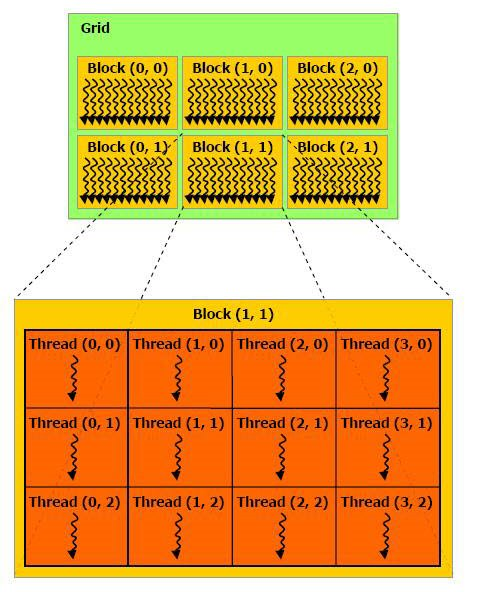
\includegraphics[width=\textwidth]
{images/Maths_Project_Presentation_gridofthreadblocks.JPG}
  \end{column}
 \end{columns}
\end{frame}

\begin{frame}{Memory Hierarchy}
 \begin{columns}
  \begin{column}{0.5\textwidth}
   In order from highest latency, lowest bandwidth and highest memory capacity (or in order of what you should minimize calls to/from):
   \begin{itemize}
    \item Host Memory
    \item Global and Local Memory
    \item Shared Memory
    \item Register Memory
   \end{itemize}
   
   We have a kind of a mixture here between a shared memory and a distributed memory system.
  \end{column}
  
  \begin{column}{0.5\textwidth}
   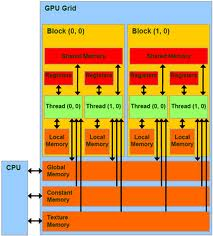
\includegraphics[width=\textwidth]
{images/Maths_Project_Presentation_memory_hierarchy.jpg}
  \end{column}
 \end{columns}
\end{frame}

%#################################################
%#	Some Performance Considerations		##
%#################################################
\subsubsection{Some Performance Considerations}

\begin{frame}{Some Performance Considerations}
 \begin{itemize}
  \item Bandwidth
  \item Latency
  \item Branch Divergence
  \item Warp Serialization
  \item Register Use
  \item Instructions Actually Used
  \item Unnecessary Extra Instructions
  \item Launch Overhead
 \end{itemize}
\end{frame}

%#########################
%#	The Solution	##
%#########################
\section{The Solution}
\subsection{Statement Of The Problem}

\begin{frame}{Statement Of The Problem}
\[
C_{ij}(\delta) = \sum_t \tr{\Phi_i(t+\delta) \tau(t+\delta, t) \Phi^\dagger_j(t) \tau(t, t+\delta) }
\]
We use
\[
\tau(t, t+\delta) = \gamma_5 \tau^\dagger(t+\delta, t) \gamma_5
\]
with $\gamma_5$ sparse (and so, easily hard coded into our kernel) and $\gamma_5 = \gamma_5^\dagger$
\end{frame}

\begin{frame}{Statement Of The Problem}
The final form of our equation is
\[
C_{ij}(\delta) = \sum_t \tr{\Phi_i(t+\delta) \tau(t+\delta, t) (\gamma_5 \tau(t+\delta, t) \gamma_5 \Phi_j(t))^\dagger }
\]
We will break down our solution as follows:
\begin{align*}
X_i^L(t, \delta)
	&= \Phi_i(t+\delta) \tau(t+\delta, t)\\
%
X_j^R(t, \delta)
	&= \gamma_5 \tau(t+\delta, t) \gamma_5 \Phi_j(t)\\
%
C_{ij}(t, \delta)
	&= \tr{ X_i^L(t, \delta) (X_j^R(t, \delta))^\dagger }\\
%
C_{ij}(\delta)
	&= \sum_t C_{ij}(t, \delta)
\end{align*}
\end{frame}

\begin{frame}{Statement Of The Problem}
 We need:
 \begin{itemize}
  \item Matrix multiplication kernel
  \item Matrix and $\gamma_5$ multiplication kernel
  \item Tracing kernel
 \end{itemize}
\end{frame}


%#########################
%#	Kernels		##
%#########################
\subsection{Kernels}

%#################################
%#	Matrix Multiplication	##
%#################################
\begin{frame}{Matrix Multiplication}
 \begin{columns}
  \begin{column}{0.5\textwidth}
   We use a tiled multiplication algorithm.
   
   \begin{itemize}
    \item $n \times n$ tile reduces global memory bandwidth by a factor $n$, moving these calls to overlapping data to shared memory.
    \item Facilitates coalescing
   \end{itemize}
  \end{column}
  \begin{column}{0.5\textwidth}
   \includegraphics[width=\textwidth]%
{images/Maths_Project_Presentation__multiply.png}
  \end{column}
 \end{columns}
\end{frame}

\begin{frame}{Comparisons}
 We use a $16 \times 16$ tile, for our tiled algorithm. Reasons include its size being a multiple of the warp size, it being the largest square tile that will run on the card and generally not being a bad number to work with.
 \begin{CUDAtiming}
  CUBLAS & 219.45\\
  \\
  Na{\"\i}ve & 34.09\\
  Tiled & 177.71\\
  \pause
  Tiled + Extras & 224.17\\
  \pause
  \\
  Fused & 266.58\\
  Fused Double Double & 298.28
 \end{CUDAtiming}
\end{frame}

\begin{frame}{Matrix and $\gamma_5$ Multiplication}
 \begin{itemize}
  \item $\gamma_5$ is sparse.
  \item Looks like a unit matrix with left half swapped with right half.
  \item Multiplication on both sides by $\gamma_5$ can be implemented with 2 or 3 extra lines of code in regular matrix multiplication.
  \item Performance impact of extra lines negligible.
 \end{itemize}
 
\end{frame}

\begin{comment}
\begin{frame}{Further Improvements}
 In our case, we can make a further improvement.

\vspace{1em}

{\bf Global Memory Bandwidth\\}
 \begin{itemize}
  \item We have multiple $\Phi$ matrices multiplying the same $\tau$ matrix.
  \item We can remove some overlapping calls to $\tau$ in global memory.
 \end{itemize}

\vspace{1em}

{\bf Parallelism\\}
 \begin{itemize}
  \item We have a known amount of the above operations to do that can be run in parallel.
  \item We can incorporate all of them into the same kernel, reducing launch overhead and increasing the number of blocks running simultaneously.
 \end{itemize}
\end{frame}

\begin{frame}{Further Improvements}
 We write two different fused kernels
 
 \vspace{1em}
 
 \begin{itemize}
  \item One simply incorporates the Parallelism ideas.
  \item The other incorporates the Parallelism and Global Memory Bandwidth ideas described above, multiplying 2 matrices simultaneously, and doing this twice in the same thread.
 \end{itemize}
 
 \vspace{1em}
 
 As such, the first has no constraint on the number of matrices to be multiplied, while the second requires it to be a multiple of 4.
\end{frame}

\begin{frame}{Comparisons}
 \begin{CUDAtiming}
  CUBLAS & 219.45\\
  \\
  Na{\"\i}ve & 34.09\\
  Tiled & 177.71\\
  Tiled + Extras & 224.17\\
  \pause
  \\
  Fused & 266.58\\
  Fused Double Double & 298.28
 \end{CUDAtiming}
\end{frame}
\end{comment}

%#################################
%#	Tracing Kernels		##
%#################################
\begin{frame}{Tracing Kernels}
 We have a problem: Tracing.
 
 \begin{itemize}
  \item $N^2$ operation. We have $c^2$ of them.
  \item Looks like a dot product, when performed on $A(B)^\dagger$ between a flattened $A$ and the conjugate of a flattened $B$, as C would flatten them.
  \item There is no piece of data in either matrix called twice, as there would be in matrix multiplication.
 \end{itemize}
 
 The result? A trace can take longer than a matrix multiplication on a CUDA card.
 
 \vspace{1em}
 
 This is ridiculous!
\end{frame}

\begin{comment}
\begin{frame}{A New Hope}
 For our problem, however, we have a lot of traces to do. Many of which use the same matrices as others.
 
 \vspace{1em}
 
 Considering a trace of two matrices can be made to look like a dot product, and considering matrix multiplications look a lot like a pile of dot products with rows being called multiple times, could we make our problem look more like a matrix multiplication?
 
 \vspace{1em}
 
 The answer: YES!
 
 \vspace{1em}
 
 Looking at it this way, it should be possible to use all the same tricks previously used in our multiplication kernel that have been tried and tested.
\end{frame}
\end{comment}

\begin{frame}{The General Idea}
 \begin{itemize}
  \item Compute each $X_i^L$ and keep them in memory such that each successively indexed matrix is next to the previous one, making one massive array.
  \item Do the exact same thing for $X_j^R$.
  \item Luckily our fastest multiplication kernels do exactly this!
  \item Multiply these together like two $c \times N^2$ matrices, assuming the right matrix is stored in a transposed format.
 \end{itemize}
 
 \vspace{1em}
 
 \begin{center}
  That is all.
 \end{center}
\end{frame}

\begin{frame}{Comparisons}
We look at a comparison of tracing kernels where the left matrix is entered as usual, but the right matrix is assumed to be in its transposed form, for reasons of coalescing and ease of programming.

 \begin{CUDAtiming}
  Na{\"\i}ve & 5.66\\
  \pause
  Tiled & 41.83\\
  \pause
  Tiled + Extras & 154.01
 \end{CUDAtiming}
\end{frame}



\section{Overall Result}

\begin{frame}{Some results}
 Using the data given, and the kernels we've built, we can get some nice results.
 
 \begin{center}
 \begin{figure}
  \subfigure[$\gamma_5$]{
   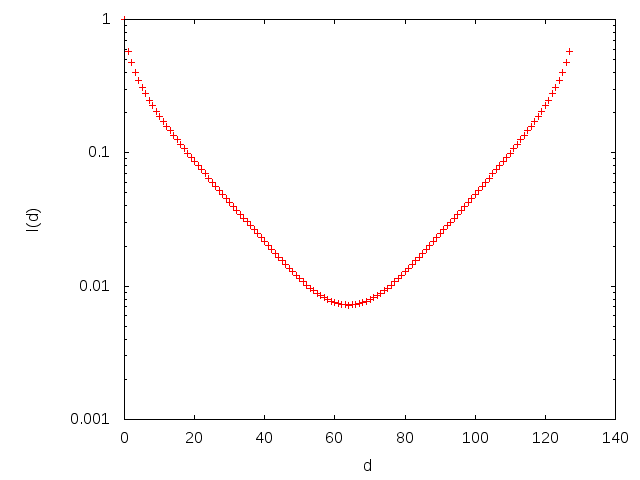
\includegraphics[width=0.3\textwidth]
{images/Maths_Project_G5.png}
   }
   \subfigure[$i\gamma_0\gamma_5$]{
    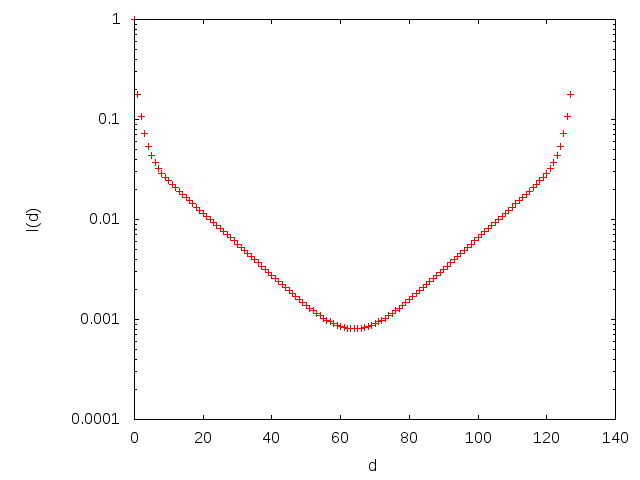
\includegraphics[width=0.3\textwidth]
{images/Maths_Project_iG0G5.png}
   }
   \subfigure[$\gamma_5$ and $i\gamma_0\gamma_5$]{
    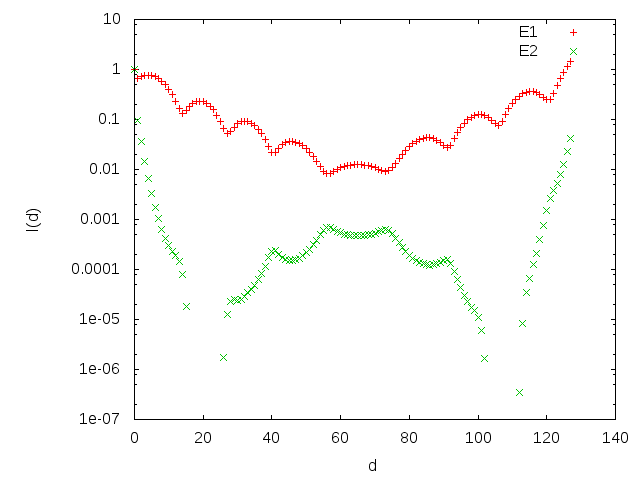
\includegraphics[width=0.3\textwidth]
{images/Maths_Project_iG0G5_G5.png}
   }
  \end{figure}
 \end{center}
 
 I've obviously made a mistake somewhere in the program, but it's nothing a good debugging can't handle. There's probably just a small indexing mistake somewhere. However, the program works approximately correctly.

\end{frame}

\begin{frame}{Some timing}

 Performing some timing tests using the "time" command, we find the following results:

 \begin{center}\begin{tabular}{l | r}
  Correlator Width & Wall Clock (s)\\
  %\hrule
  $1 \times 1$ & 230\\
  $2 \times 2$ & 235\\
  $15 \times 15$ & 1301\\
  $16 \times 16$ & 598\\
  $17 \times 17$ & 758\\
  $32 \times 32$ & 967\\
  $64 \times 64$ & 1701
 \end{tabular}\end{center}

 Compare this to the (admittedly crappy) serial code I wrote to do the same, which took 344~s for a $1 \times 1$ correlator with a time length of only 4, versus the 128 for the above correlators.

\end{frame}


\begin{frame}{Future developments}

 \begin{itemize}
  \item Need to do some debugging!

  \item What else can this approach be used for?
 
 Baryon contraction: 
 $
 \Phi_{abc} \tau_{a\bar{a}} \tau_{b\bar{b}} \tau_{c\bar{c}} \Phi_{\bar{a}\bar{b}\bar{c}}
 $
 
  \item ????
 
  \item Profit!
 \end{itemize}

\end{frame}

\begin{frame}{The End}
\begin{center}
Thank you for your attention!

Any questions?
\end{center}
\end{frame}


\end{document}